\question 下列关于传输层协议中面向连接的描述,( )是错误的
\par\fourch{面向连接的服务需要经历3个阶段:连接建立、数据传输以及连接释放}{面向连接的服务可以保证数据到达的顺序是正确的}{\textcolor{red}{面向连接的服务有很高的效率和时间性能}}{面向连接的服务提供了一个可靠的数据流}
\begin{solution}由于面向连接的服务需要建立连接,并且需要保证数据的有序性和正确性,导致了它比无连接的服务开销大,而速度和效率方面也比无连接的服务差一点。
\end{solution}
\question 假设某应用程序每秒产生一个60B的数据块,每个数据块被封装在一个TCP报文中,然后再封装到一个IP数据报中,那么最后每个数据报所含有的应用数据所占的百分比是(
)(注意:TCP报文和IP数据报的首部没有附加字段)
\par\twoch{20\%}{40\%}{\textcolor{red}{60\%}}{80\%}
\begin{solution}因为TCP报文和IP数据报的头部没有附加字段,所以一个TCP报文的头部长度为20B。一个IP数据报首部的长度也是20B,再加上60B的数据,所以一个IP数据报的总长度为100B。所以,每个数据报所含有的应用数据所占的百分比是60\%。
\end{solution}
\question 如果主机1的进程以端口x和主机2的端口y建立了一条TCP连接,这时如果希望再在这两个端口间建立一个TCP连接,那么会
\par\fourch{\textcolor{red}{建立失败,不影响先前建立连接的传输}}{建立成功,并且两个连接都可以正常传输}{建立成功,先建立的连接被断开}{建立失败,两个连接都被断开}
\begin{solution}一条连接使用它们的套接字来标识,因此(1,x)-(2,y)是在两个端口之间唯一可能的连接。而后建立的连接会被阻止,并不影响先前已经存在的连接。
\end{solution}
\question 下列说法正确的是( )。
Ⅰ.传输层是OSI模型的第四层,是整个网络协议体系的核心
Ⅱ.传输层传输数据只能在源主机和目的主机之间进行点到点的传输
Ⅲ.TCP和UDP是典型的传输层协议,TCP是面向连接的,而UDP是面向无连接的
Ⅳ.TCP连接进行流量控制和拥塞控制,而UDP既不进行流量控制,又不进行拥塞控制
\par\twoch{Ⅰ、Ⅱ、Ⅲ}{Ⅰ、Ⅱ、Ⅳ}{\textcolor{red}{Ⅰ、Ⅲ、Ⅳ}}{Ⅱ、Ⅲ、Ⅳ}
\begin{solution}传输层实现的是端到端的传输,即实现进程之间的通信,故Ⅱ错误,Ⅰ、Ⅲ、Ⅳ正确。
\end{solution}
\question 下列关于TCP的叙述中,正确的是( )。 Ⅰ.TCP是一个点到点的通信协议
Ⅱ.TCP提供了无连接的可靠数据传输
Ⅲ.TCP将来自上层的字节流组织成IP数据报,然后交给IP
Ⅳ.TCP将收到的报文段组成字节流交给上层
\par\twoch{Ⅰ、Ⅱ、Ⅳ}{Ⅰ、Ⅲ}{\textcolor{red}{仅Ⅳ}}{Ⅲ、Ⅳ}
\begin{solution}TCP在网络层IP的基础上,向应用层提供可靠、全双工的端到端的数据流传输,所以TCP是一个端到端的通信协议,而IP才是点到点的通信协议,因此Ⅰ、Ⅱ错误。TCP通过可靠的传输连接将收到的报文段组织成字节流,然后交给上层的应用进程,这就为应用进程提供了有序、无差错、不重复和无报文丢失的流传输服务,Ⅳ正确。IP数据报不是由传输层组成的,而应该由网络层加上IP数据报的首部来形成IP数据报,Ⅲ错误。
\end{solution}
\question 下列关于TCP和UDP的描述正确的是( )。 Ⅰ.TCP和UDP都是无连接的
Ⅱ.TCP是无连接的,UDP是面向连接的
Ⅲ.TCP适用于可靠性较差的网络,UDP适用于可靠性较高的网络
Ⅳ.TCP适用于可靠性较高的网络,UDP适用于可靠性较差的网络
\par\twoch{Ⅱ、Ⅳ}{Ⅱ、Ⅲ}{Ⅳ}{\textcolor{red}{Ⅲ}}
\begin{solution}TCP是面向连接的,UDP是无连接的,故Ⅰ、Ⅱ错误。由于TCP是可靠的传输,即使网络本身性能比较差,TCP也能保证较好的性能,故适用于可靠性比较差的网络;而UDP是不可靠的传输,如果网络本身还不可靠,就会造成错误太多,故UDP适用于可靠性较高的网络,Ⅲ正确,Ⅳ错误。
\end{solution}
\question 下列关于TCP协议的叙述,正确的是
\par\fourch{TCP是一个点到点的通信协议}{TCP提供了无连接的可靠数据传输}{TCP将来自上层的字节流组织成IP数据报,然后交给IP协议}{\textcolor{red}{TCP将收到的报文段组成字节流交给上层}}
\begin{solution}TCP协议在网络层IP协议的基础上,向应用层提供可靠、全双工的端到端的数据流传输。TCP协议通过可靠的传输连接将收到的报文段组织成字节流,然后交给上层的应用进程,这就为应用进程提供了有序、无差错、不重复和无报文丢失的流传输服务。A选项IP协议才是点到点的通信协议,C选项中IP数据报不是由传输层来组成的,而应该由网络层加上IP数据报的首部来形成IP数据报。
\end{solution}
\question 下列关于TCP和UDP的描述,正确的是
\par\twoch{TCP和UDP都是无连接的}{TCP是无连接的,UDP是面向连接的}{\textcolor{red}{TCP适用于可靠性较差的网络,UDP适用于可靠性较高的网络}}{TCP适用于可靠性较高的网络,UDP适用于可靠性较差的网络}
\begin{solution}显然A、B错误。由于TCP是可靠的传输,所以适用于可靠性比较差的网络;而UDP是不可靠的传输,如果网络本身还不可靠,就会造成错误太多,所以UDP适用于可靠性较高的网络。
\end{solution}
\question 主机甲向主机乙发送一个(SYN=1,seq=11220)TCP段,期望与主机乙建立TCP连接,若主机乙接受该连接请求,则主机乙向主机甲发送的正确的TCP段可能是(
)
\par\fourch{(SYN=0,ACK=0,seq=11221,ack=11221)}{(SYN=1,ACK=1,seq=11220,ack=11220)}{\textcolor{red}{(SYN=1,ACK=1,seq=11221,ack=11221)}}{(SYN=0,ACK=0,seq=11220,ack=11220)}
\begin{solution}首先,不管是连接还是释放,一般只要写出来,SYN、ACK、FIN的值一定是1,排除A和D选项。确认号是甲发送的序列号加1,ACK的值应该为11221(即11220已经收到,期待接收11221)。另外需要重点提醒的是,乙的SEQ值是主机随意给的,和甲的SEQ值没有任何关系,这里只是巧合。
【总结】
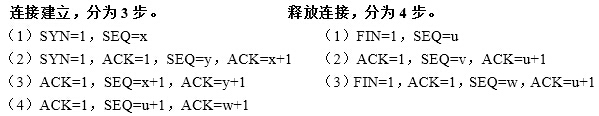
\includegraphics[width=6.23958in,height=1.20833in]{computerassets/0349051efcbc98e2d82b387bf89b9028.jpeg}
【提醒】
在连接建立中,第一步其实也有ACK的值,且值为0;第三步中也有SYN的值,其值也为0,但是都可以省略不写,所以一般写出来的值都一定是1(考生可参考2012年真题第47题的数据)。
\end{solution}
